\documentclass[12pt]{book}
\usepackage[inner=1.25in, outer=1in, top=1in, bottom=1in]{geometry}
\title{Automated Attendance System}
\author{Govind M J}
\usepackage{graphicx}
\usepackage[document]{ragged2e}
\usepackage{titlesec}

\titleformat{\chapter}[display]
{\normalfont\bfseries}{}{0pt}{\Huge}


\setlength{\parindent}{0pt}
\begin{document}
	\pagestyle{plain}
    \pagenumbering{roman}
    \setlength\columnsep{20pt}
    \setlength{\columnseprule}{1pt}
	\centering
    \huge
    \thispagestyle{empty}
    \textbf{Progress Report Book} \vfill
    \large
    \textbf{On} \vfill
    \huge
    \textbf{Automated Attendance System}
    \LARGE \\[10pt]
    \textbf{19-202-0611 Mini Project} \vfill
    \vfill
    \large
    \textbf{By} \\ [6pt]
    \Large
   	27 - A S Swan \\
    42 - Govind M J \\
    51 - Joel John Varghese \\
    55 - Lakshmi Manoj \vfill
    
    \Large
    (B.Tech. Computer Science and Engineering - Batch A) \vfill
    \textbf{Under the Guidance of} \\[6pt]
    Dr. Sheena Mathew \vfill
    

    \vfill
    
    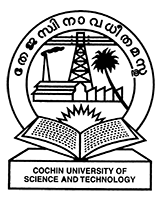
\includegraphics[width=0.20\textwidth]{./logo.png}\\[0.5cm]
    \textbf{School of Engineering\\ Cochin University of Science and Technology} \\
    [10pt]
    2023 \\
    
    \chapter*{Preface}
    \normalsize
    \paragraph{}
    
    \begin{flushleft}
    	This progress report book provides a comprehensive overview of the development and implementation of the attendance management system. The goal of this project is to create a user-friendly system for tracking student attendance, enabling teachers and administrators to easily view attendance records and generate reports. The system is web-based, allowing users to access it from any device with an internet connection. \\[6pt]
    	
    	The project team consists of four individual. Our team is committed in delivering a high-quality system that meets the needs of attendance management. \\[6pt]
    	
    	This progress report book will provide an overview of the project's objectives, scope, methodology, and deliverables. We will also discuss the challenges encountered during the development process, and the strategies implemented to overcome them. In addition, we will provide a detailed description of the system's features, including the user interface, data management, security, and reporting capabilities. \\[6pt]
    	
    	We hope that this progress report book will serve as a valuable resource, providing insight into the development process and the system's functionality.
    \end{flushleft}
    
    
    
    \tableofcontents


    \chapter{Week 1}
    \justifying
    \large
    08/03/2023 \\[10pt]
    
    
    \pagenumbering{arabic}
    \setcounter{page}{1}
    	
    \paragraph{}
    There are several distinct phenomena which can be used to measure mass. Although some theorists have speculated that some of these phenomena could be \textbf{independent of each other}, current experiments have found no difference in results regardless of how it is measured:
    
    - Inertial mass measures an object's resistance to being accelerated by a force (represented by the relationship F = ma).
    - Active gravitational mass measures the gravitational force exerted by an object.
    - Passive gravitational mass measures the gravitational force exerted on an object in a known gravitational field.
    
    \chapter{Week 2}
    \justifying
    \large
    15/03/2023 \\[10pt]
    
    \paragraph{}
    There are several distinct phenomena which can be used to measure mass. Although some theorists have speculated that some of these phenomena could be \textbf{independent of each other}, current experiments have found no difference in results regardless of how it is measured:
    
    - Inertial mass measures an object's resistance to being accelerated by a force (represented by the relationship F = ma).
    - Active gravitational mass measures the gravitational force exerted by an object.
    - Passive gravitational mass measures the gravitational force exerted on an object in a known gravitational field.
    
    %Add Next weeks here!!!
    
\end{document}
